


%%%%%%%%%%%%%%%%%%%%%%%%%%%%%%%%%%%%%%%%%%%%
\section{Simulating Ultrasound-Guidance Interventions}


%%%%%%%%%%%%%%%%%%%%%%%%%%%%%%%%%%%%%%%%%%%%%%%%%%%%%%%%
{
\paper{Wright-Gilbertson M. 2014 in PhD thesis: Xia et al., 2017 in Scientific Reports}
\begin{frame}{The sonographer-probe-patient control system}
      \begin{figure}
        \centering
        \includegraphics[width=1.0\textwidth]{./../figures/sonographer-probe-patient/versions/drawing-v02.png}
        %\caption{}
      \end{figure}
\end{frame}
}





%%%%%%%%%%%%%%%%%%%%%%%%%%%%%%%%%%%%%%%%%%%%%%%%%%%%%%%%%
%{
%\paper{(a) Coordinate systems overview sketch in 3D Slicer,  (b) Asselin et al. 2018 in conf-BIVPCS, (c) US-simulator, and (d) 3D-printed fetus}
%\begin{frame}{Simulator for Ultrasound-Guidance Interventions}
%
%  \begin{columns}
%    \begin{column}{.3\linewidth}
%      Towards a more realistic
%  \begin{itemize}
%    \item \textbf{UGI}
%    \item \textbf{US images}
%    \item \textbf{Phantoms with 3D-printed US compatible material}
%    \item \textbf{Training for in-plane, out-of-plane needle tracking}
%  \end{itemize}
%
%    \end{column}
%
%
%  \begin{column}{.6\linewidth}
%
%      \begin{figure}
%        \centering
%        \includegraphics[width=0.9\textwidth]{./figures/sugi/plan-simulator-for-ugi/versions/drawing-v02.png}
%      \end{figure}
%
%    \end{column}
%  \end{columns}
%
%\end{frame}
%}